\chapter{Konzept}

(Joshua)

In diesem Kapitel soll beschrieben werden, wie die in \autoref{sec:frameworks} beschriebenen Frameworks und Technologien in diesem Projekt zusammen spielen sollen. Hierzu wird zum einen auf die Architektur des Servers, der die API zur Verfügung stellt, eingegangen und zum anderen beschrieben wie der mobile Client aufgebaut ist. Als letztes wird aufgezeigt, wie beide Applikationen miteinander kommunizieren.

	\section{Kommunikationsschema}
	Da bei diesem Projekt zwei unabhängige Applikationen entstehen (zum einen der mobile Client und zum anderen der Server), ist es sehr wichtig die Schnittstelle zwischen beiden möglichst früh festzulegen. Zudem ist es möglich aus der Beschreibung der Schnittstelle ein Code-Gerüst zu generieren, siehe \autoref{sec:swagger}. Aus diesen Gründen wurde entschieden mit dem Kommunikationsschema zu beginnen.
	
	\subsection{Entitäten}\label{sec:entities}
	
	Die entstandene Swagger Beschreibung der API beinhaltet die grundlegende Struktur der Entitäten, die in unserer Applikation genutzt werden sollen. Dazu zählen unter anderem:
	
	\begin{itemize}
		\item \textbf{Stop:} Die \acs{POI}s, die dem Nutzer angezeigt und zur Auswahl gestellt werden sollen werden in der Stop Entität gespeichert und kommuniziert. Diese Entität beinhaltet alle notwendigen Informationen, wie den Namen des interessanten Punktes, die geografische Lage und die Kategorie, welchem der Punkt zugeordnet ist. Des Weiteren sind Informationen zu Bewertungen enthalten, die von Nutzern abgegeben wurden. Damit bildet die Stopentität die Grundlage für einen \textit{Trip}, welcher aus einer Folge von \textit{Stops} aufgebaut ist. 
		
		\newpage
		
		\begin{figure}[ht!]
			\centering
			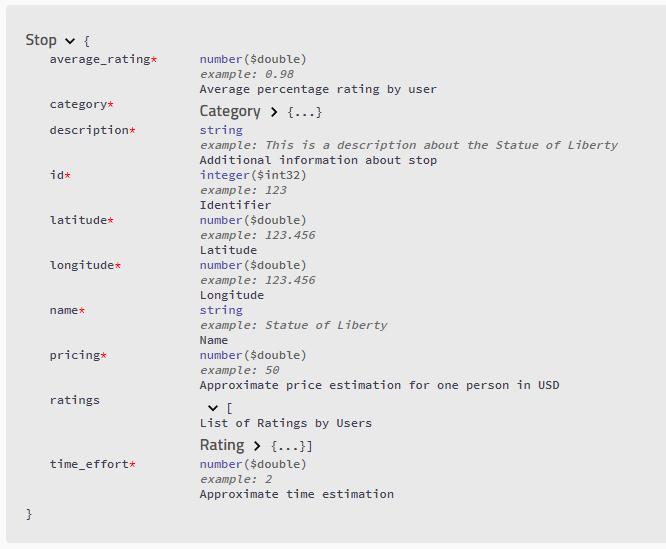
\includegraphics[width=1\textwidth]{images/swagger_stop_entity.png}
			\caption{Swaggerbeschreibung der Stopentität}
			\label{fig:swagger_stop}
		\end{figure} 
		
		\autoref{fig:swagger_stop} zeigt für die Stop Entität beispielhaft, wie eine Entitätsbeschreibung auf dem von Swagger bereitgestellten UI aussieht. Alle Elemente, die mit einem roten Stern gekennzeichnet sind, sind zwingend erforderlich um eine solche Entität anzulegen. Für jedes Attribut ist eindeutig festgelegt, welchen Typ es hat, ein Beispiel und eine kurze Beschreibung, welche die Benutzung erleichtern soll. Wie an den Attributen \textit{category} und \textit{ratings} zu erkennen, können die einzelnen Entitäten untereinander Verschachtelt werden, um eine konsistente und vollständige Typisierung zu erreichen.   
		\item \textbf{Trip:} Ein \textit{Trip} ist wie bereits erwähnt eine Abfolge von Stop Entitäten. Entsprechend ist der zentrale Bestandteil einer Trip Entität eine Sammlung von Stop Entiäten. Daneben gibt es weitere Informationen zu der zugeordneten Stadt, zum Veröffentlichungsstatus des Trips und zu ggf. vorliegenden Ratings.
		\item \textbf{City:} Jede Stadt, welche in \textit{Travlyn} besucht werden kann, wird in einer City Entität gespeichert. Diese Entität beinhaltet Informationen wie Name, Beschreibung und ein die Adresse eines aussagekräftigen Bildes der Stadt. Einer Stadt sind alle in dieser Stadt liegenden Trips zugeordnet. 
		\item \textbf{User:} Die User Entität beinhaltet alle klassischen Informationen zu einem Benutzer der App, dazu zählen z.B. seine E-Mail Adresse, seine technische ID und sein Name. Vor allem für das in  \autoref{sec:funcReq} beschriebene Nutzungsprofil \textit{Registered User} ist diese Entität von zentraler Bedeutung, da eine Identifizierung des Nutzers notwendig ist um Trips zu speichern oder persönlich zugeordnete Informationen anzulegen und zu verwalten.
	\end{itemize}

	Neben den hier beschriebenen Entitäten gibt es noch einige weitere kleinere Entitäten in diesem Projekt, wie z.B. das \textit{token} oder wie bereits in der Stop Entität verwendet das \textit{rating} und die \textit{category}. Diese Entitäten und alle genaueren Beschreibungen (wie \autoref{fig:swagger_stop}) sind im Sinne der Übersichtlichkeit nicht dargestellt, können aber bei Abruf der API eingesehen werden \footnote{\url{https://travlyn.raphael-muesseler.de/travlyn/travlyn/1.0.0/swagger-ui.html}}.
	
	\subsection{Requests}
	
	Neben den beschriebenen Entitäten beinhaltet die Swaggerbeschreibung Schemata, wie bestimmte Informationen von der API abgerufen werden können. Diese Beschreibung bietet jedem die Möglichkeit die API zu erkunden und schreibt damit genau vor, welche Services der Server bereitstellen muss aber auch wie der Client bestimmte Informationen erfragen kann.
	
	\vspace{0.25cm}
	
	Im Folgenden wird einer der Requests genauer beschreiben und die entsprechenden Elemente im von Swagger bereitgestellten UI gezeigt. Neben diesem beispielhaften Request gibt es viele weitere Requests mit unterschiedlichsten Spezifikationen, welche bei Bedarf auf der in \autoref{sec:entities} bereits beschriebenen Website Abgerufen werden können und sogar mit direktem Zugriff auf die implementierte API getestet werden können.
	\begin{itemize}
		\item \textbf{/stop/\{stopId\}:} Durch die Angabe einer technischen \textit{stopId} kann über diese Schnittstelle eine Stop Entität zu erfragen. Im Swagger UI wird der Request mit seiner Beschreibung und allen erforderlichen Parametern angezeigt.  
		
		\begin{figure}[ht!]
			\centering
			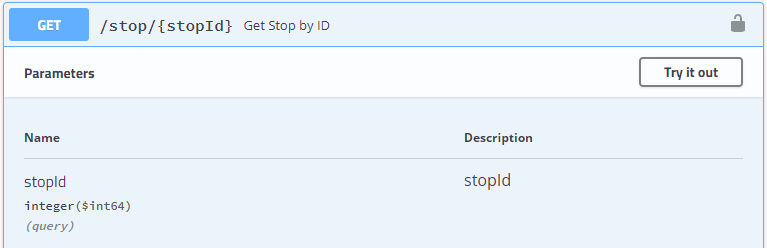
\includegraphics[width=1\textwidth]{images/swagger_getStop_head.png}
			\caption{Beschreibung des \textit{getStop} Requests im Swagger UI}
			\label{fig:swagger_getStop_head}
		\end{figure} 
		
		Außerdem werden die möglichen Antworten der API auf diesen Request angezeigt, um zu verdeutlichen was der Client genau zu erwarten hat und welche Fehler bei der Benutzung der Schnittstelle auftreten können.
		
		\begin{figure}[ht!]
			\centering
			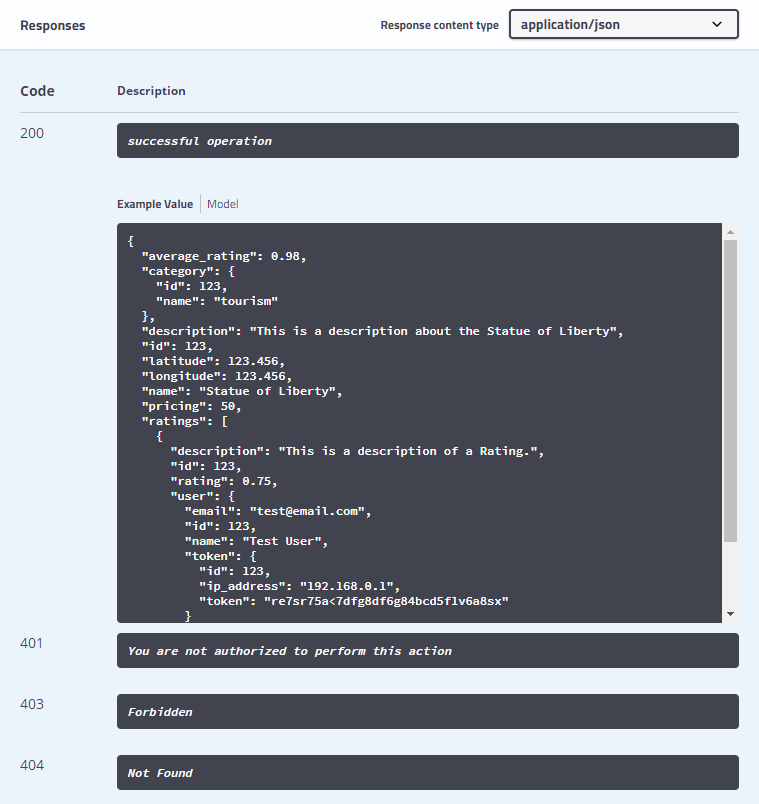
\includegraphics[width=1\textwidth]{images/swagger_getStop_response.png}
			\caption{Beschreibung des \textit{getStop} Requests im Swagger UI}
			\label{fig:swagger_getStop_response}
		\end{figure}
	
	Wie in \autoref{fig:swagger_getStop_response} zu sehen wird die Antwort im \acs{JSON} Format zurückgegeben, falls kein Fehler aufgetreten ist. In diesem Fall ist eine Antwort im selben Format zu erwarten, wie unter \enquote{Example Value} dargestellt. Dies ist die \acs{JSON} Darstellung der bereits vorgestellten Stop Entität (siehe \autoref{sec:entities}). Es sind alle Attribute, wie z.B. die Id oder der Name des \acs{POI}, wiederzuerkennen und in diesem Fall mit den gleichen Beispielwerten belegt, die in der Entitätsbeschreibung festgelegt wurden. Neben der erfolgreichen Antwort mit \acs{HTTP} Code 200 sind alle Fehlercodes, die von der API zurückgegeben werden können kurz beschreiben. Zusätzlich zu den hier gezeigten Codes ist der Code 500 (\textit{Internal Server Error}) zu berücksichtigen, welcher immer auftreten kann.
	
	\newpage
	
	\end{itemize}
		
	\section{Server Architektur}
	
	Wie in \autoref{sec:swagger} beschrieben ist es möglich aus der oben beschriebenen Swagger Beschreibung ein komplettes Code-Gerüst für eine Spring Applikation zu generieren. Diese Funktionalität wurde sich für das vorliegende Projekt zunutze gemacht. Damit entstand eine Spring Applikation, welche die in \autoref{sec:spring} beschriebenen Patterns verwendet und implementiert.
	
	\vspace{0.25cm}
	
	In \autoref{fig:UML} ist eine Übersicht über die grobe Struktur der Server Applikation zu sehen. Dieses UML Diagramm ist stark vereinfacht und beinhaltet nur beispielhafte Klassen, die symbolisch für einen größeren Verbund stehen sollen. So existiert wie bereits beschreiben nicht nur die Stop API und die dazugehörigen Interfaces und Klassen sondern noch viele weitere wie z.B. die User oder Trip API. Trotzdem ist erkennbar, dass sich die Serverarchitektur in mehrere Bereiche aufteilen lässt:
	
	\begin{itemize}
		\item \textbf{Spring-Klassen:} Zur Nutzung von Spring werden einige Klassen benötigt, um bestimmte Konfigurationen und Dienstprogramme aufzusetzen. Diese Klassen werden an sehr vielen Stellen über \textit{Dependency Injection} (siehe \autoref{sec:spring}) in Spring und andere Teile der Architektur eingebunden. Besonders hervorzuheben ist an dieser Stelle die Klasse \textit{TravlynServer}, welche die Methode enthält, um die komplette Springapplikation zu starten.
		\item \textbf{Controller:} Controller liegen ebenfalls unter starker Kontrolle des Spring Frameworks. Alle Requests, die auf der API eingehen werden von Spring an den entsprechenden Controller übergeben. Diese sind für die Verarbeitung der Anfragen verantwortlich und extrahieren Parameter, allerdings beinhalten sie keinerlei Businesslogik, sondern delegieren die Aufgaben an die zentrale Serviceklasse. Diese ist ebenfalls über \textit{Dependency Injection} eingebunden, um die Verwaltung der Beziehung dem Framework zu überlassen. Nach der Ausführung der Anfrage werden die entsprechenden Informationen zurückgegeben und für eine entsprechende \acs{HTTP}-Antwort gesorgt. Durch dieses Verfahren können serverinterne Informationen wie detaillierte Fehlernachrichten vor dem Nutzer der API versteckt werden, um Angriffe zu erschweren.
		
		Neben der funktionalen Bedeutung für die Anwendung beinhalten die Controller Dokumentation entsprechend zu der Swagger-Beschreibung. Diese sorgt dafür, dass die \textit{Travlyn} API selbständig von Nutzern erkundet werden kann.
		\item  \textbf{Service:} Die Klasse \textit{TravlynService} ist das Herzstück des Servers und beinhaltet die meiste Businesslogik. Sie steht zum Teil unter der Kontrolle des Spring Frameworks, muss aber komplett händisch implementiert werden. In dieser Klasse werden alle Operationen, die der Server ausführen muss (z.B. Login eines Nutzers, Sammeln der POI's für eine Stadt oder erzeugen eines Trips) implementiert. Diese Klasse hält alle anderen Komponenten, wie die Controller, den Datenbankzugriff und weitere externe Funktionalitäten zusammen und kontrolliert ihr zusammenwirken.
		\item  \textbf{DTOs und Entitäten:} Auf dem Server werden Objekte in zwei unterschiedlichen Formaten gehalten, welche nicht unter der Kontrolle vom Spring aber zum Teil unter der Kontrolle von Hibernate stehen. Zum einen existieren sog. \ac{DTO}s. Diese beinhalten ausschließlich die Inforationen, die als Ergebnis einer API-Abfrage übermittelt werden. Zum anderen sind Datenentitäten entstanden, wie sie von Hibernate genutzt werden. Die Entitäten besitzen die gleiche Struktur, wie die zugrundeliegenden Datenbanktabellen und damit alle vorliegende Informationen. Dieses Pattern wird genutzt um bestimmte Informationen zu verstecken und eine Trennung zwischen der Sicht des Servers auf die Daten und der Sicht des API Nutzers zu erreichen. In der Literatur wird dieses Pattern als \textit{Interface Segregation Principle} genannt und ist Teil des \textit{SOLID} Konzepts \cite{GOLL.2019}. Beide Objekttypen sind über entsprechende Methoden ineinander umwandelbar.
		\item \textbf{Hilfsklassen:} Neben allen bereits genannten Funktionalitäten müssen weitere externe Funktionen eingebunden werden. Im Fall von \textit{Travlyn} hauptsächlich fremde \acs{API}s, die alle nötigen Daten zu \acs{POI}s, Städten und Karten zur Verfügung stellen. Diese Zugriffe werden im Service benötigt, um die angefragten Operationen ausführen zu können. Dieser Teil der Applikation steht nicht unter der Kontrolle eines Frameworks und wurde händisch integriert. 
	\end{itemize}
	
	
	\begin{figure}[ht!]
		\centering
		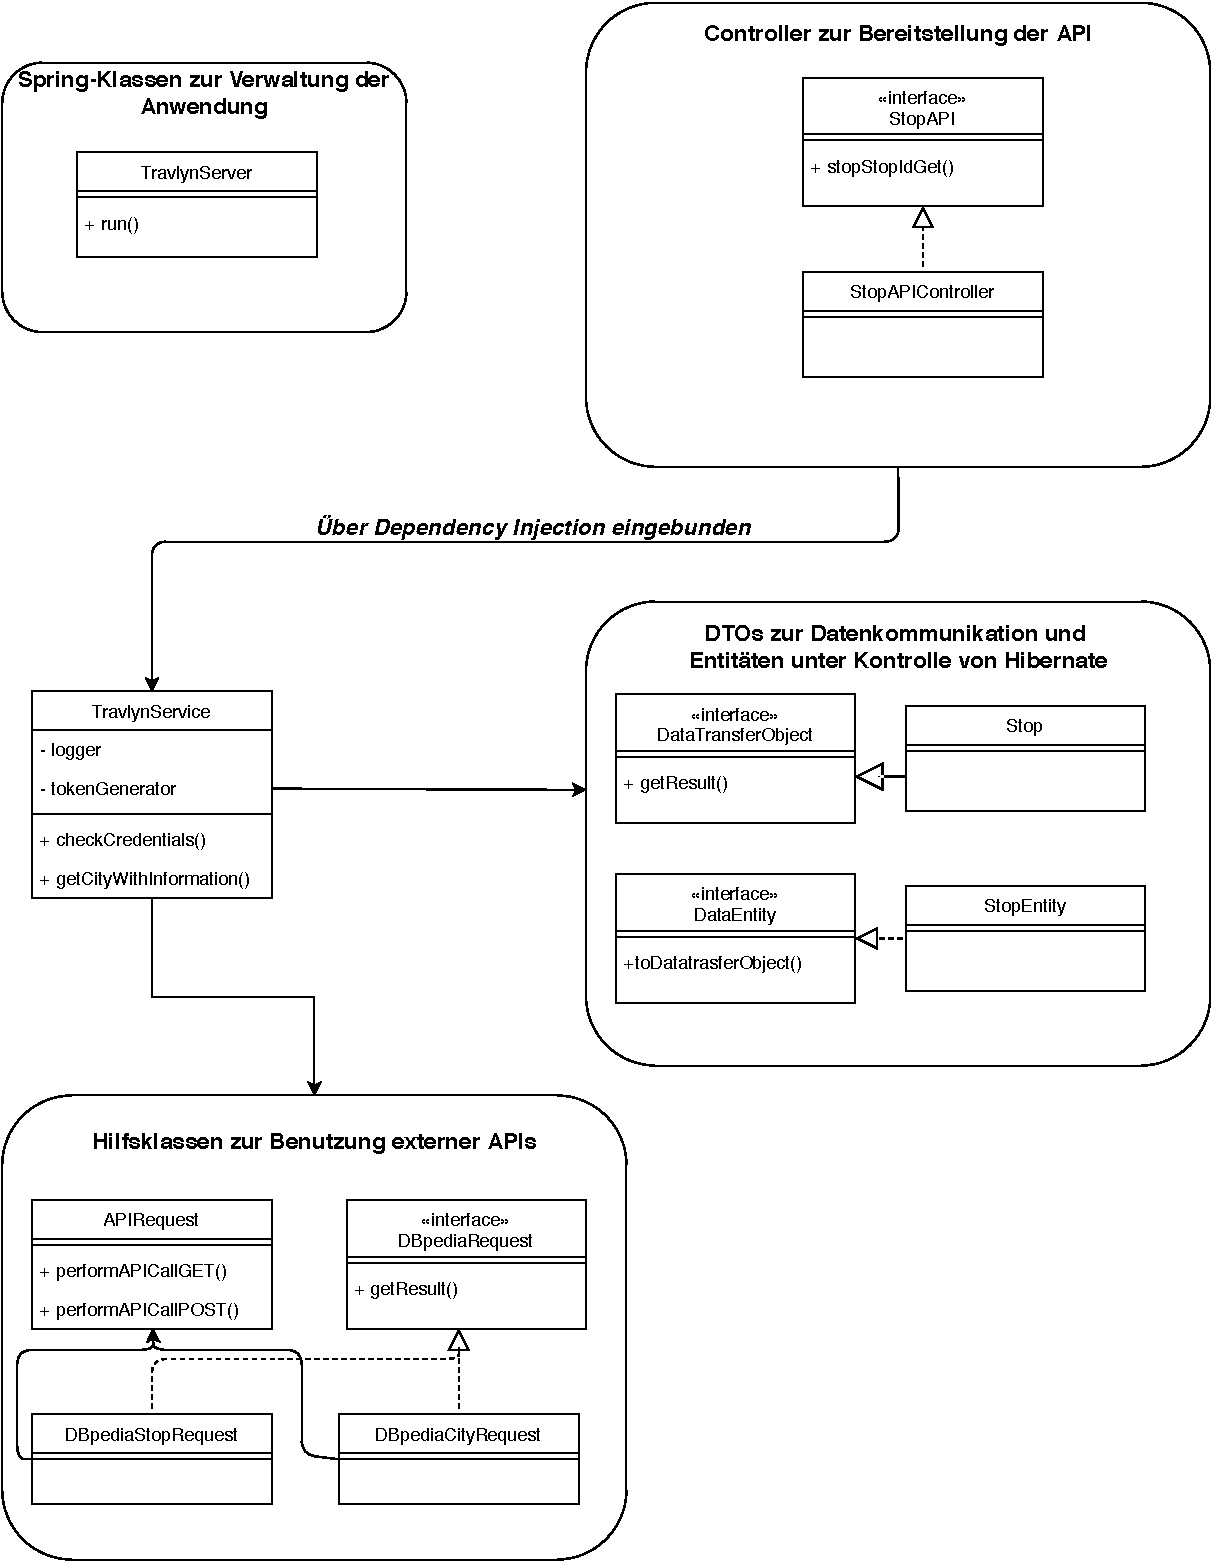
\includegraphics[width=1\textwidth]{images/UML_Diagram.pdf}
		\caption{Struktur des \textit{Travlyn} Servers als UML Diagramm. Zu Beachten ist, dass dieses Diagramm stark vereinfacht und nicht vollständig ist, um die Übersichtlichkeit zu wahren.}
		\label{fig:UML}
	\end{figure}

	\clearpage

	
	\section{Client Architektur}
		
		Neben der automatischen Generierung von Code, welcher das Spring Framework nutzt, ist es mit Swagger ebenfalls möglich, Code für den Client zu generieren. Da diese Generierung viel Arbeit und Einrichtungsaufwand spart, wurde auch das Grundgerüst für den \textit{Travlyn} Client automatisch generiert.
		
		\subsection{Model}
		
		\subsection{title}

	\section{Deployment Architektur}
	
		Wie bereits in \autoref{qm.continuous_delivery} wird der \textit{Travlyn} Server über ein Docker Image (siehe \autoref{frameworks.docker}) ausgeliefert. 
	